\section{Surface pressure and skin friction, by section}
\label{sec:app:sections}

\textbf{Purpose.} This appendix carries the surface distributions behind the integrated
coefficients in the body of the report. Every geometry is cut at five spanwise stations,
$\eta = 0.20$, $0.40$, $0.60$, $0.80$ and $0.95$, at its own trimmed incidence to that
condition's own target lift: $C_L = 0.428277635108$ at Condition~CR, $C_L = 0.529297087450$ at
early cruise and $C_L = 0.544114800210$ at late cruise, all on the DSO basis. Comparing the six geometries' $-c_p$ peaks at a station
means something only because they share that target within a condition.

\textbf{Conditions are never overlaid.} Condition~CR and cruise are normalised on different
dynamic pressures: $q = 578$ (kinematic, $\mathrm{m^2/s^2}$, the incompressible solver carries no
density) against $q = \num{11292.8}$~Pa at early cruise and $\num{8257.37}$~Pa at late cruise.
Each is correct and they are not comparable curves, so every condition is plotted as its own set
and the plotting script refuses to mix them.

\textbf{Coverage.} All three conditions are six geometries of six: $90$ station files over $18$
cases, with no case partially represented.

\textbf{What is plotted.} Figures~\ref{fig:perf:cp}, \ref{fig:perf:cp:ec} and~\ref{fig:perf:cp:lc} carry $c_p$ on an
inverted axis and its difference from the baseline by surface; Figures~\ref{fig:perf:cf}
and~\ref{fig:perf:cf:lower} carry the signed skin friction by surface. All are against $x/c$ on
the local chord of that station, which falls from $0.4816$~m at $\eta = 0.20$ to $0.1671$~m at
$\eta = 0.95$.

\textbf{The curves are a band, not a line.} The pressure and skin-friction
curves pool faces within $\pm 0.004$ semispan, $\pm 7.32$~mm, and the wing is swept and tapered,
so faces at one $x/c$ sit at different $y$ and carry genuinely different $z$; curves are the median
over $0.005c$ bins per surface rather than the raw scatter. Within one bin the $10$--$90$ percentile spread of $z/c$ is
$1.5$ to $2.3$~per~cent of chord at the leading edge, where the surface turns through nearly
$180^\circ$, and about $1.1$~per~cent at the blunt trailing edge, against $0.21$ to
$0.49$~per~cent at mid-chord. A defective surface would be ragged at mid-chord too.

\textbf{Two of the three sources of raggedness are the sampling band. The third was a defect and
is now corrected.} The leading-edge scatter is the band meeting high curvature: across the five
stations the within-bin spread grows by a factor of $2.79$ while the band's share of the local
chord grows by $2.80$, with mid-chord flat throughout as a control. That is also why the outboard
stations are the noisiest, the fixed $14.63$~mm slab spanning $3.0$~per~cent of chord at
$\eta = 0.20$ but $8.8$~per~cent at $\eta = 0.95$. The inboard trailing-edge ripple is the band
meeting taper rather than curvature: the chord shortens by $0.2279$~m per metre of span, so it
varies by $3.33$~mm across the slab and a face is binned at an $x/c$ that is not quite its own.
Neither is removable without narrowing the band, and both are sampling rather than flow. The
OUTBOARD trailing-edge ripple was neither, and it was not flow either: it was the upper-lower
split failing where the two surfaces converge. Splitting on the exported facet normals instead
removes it. Measured as the within-bin $C_p$ spread over $x/c = 0.92$ to $1.00$, C at
$\eta = 0.80$ falls from $0.2623$ to $0.0204$ and M from $0.2797$ to $0.0177$; at $\eta = 0.95$
the six cases fall from about $0.34$ to about $0.09$. Two controls hold and are what make this a
correction rather than a smoothing: mid-chord is unchanged to four decimal places, $0.0447$
against $0.0447$ for C at $\eta = 0.80$, and the inboard station is unchanged at $\eta = 0.20$,
ratio $1.03$, because the band and the taper are still there.

\textbf{The band also over-reads the local chord, by a fixed length rather than a fixed
fraction.} It takes its leading edge from the inboard face of the slab and its trailing edge from
the outboard one, so on a swept wing it over-reads by
$(w/2)(\tan\Lambda_{\mathrm{LE}} + \tan\Lambda_{\mathrm{TE}})$. With $w = 14.63$~mm,
$\Lambda_{\mathrm{LE}} = 28.84^\circ$ and $\mathrm{d}c/\mathrm{d}y = -0.266$ that predicts
$6.11$~mm against $6.67$~mm measured, and the measured excess is near-constant across span while
the chord itself halves, which is the signature of a slab width rather than of a scaling error.
The chords quoted above are the planar-cut values and are accordingly $1.4$~per~cent smaller than
the band's at $\eta = 0.20$ and $3.8$~per~cent smaller at $\eta = 0.95$. Because $x/c$ is
normalised to span $0$ to $1$, the curves are unaffected; only the dimensional chord printed
above each column of the figures differs.

\textbf{The sign on $C_{f,s}$ is the useful part.} $C_{f,s}$ is the component of wall shear
along the freestream, taken from each case's own \texttt{dragDir}, so \emph{negative means
reversed flow}. The sign convention is calibrated per case against inboard mid-chord faces whose
attachment is known independently, not assumed; it came out one-signed on all twelve cases.

\subsection{Overview at the five stations}
\label{sec:app:overview}

Figures~\ref{fig:perf:cp} to~\ref{fig:perf:cf:lower} draw the five stations of each condition on
one page each, pressure first and then skin friction by surface; the two subsections that follow
read them condition by condition.
\begin{figure}[htbp]
\centering
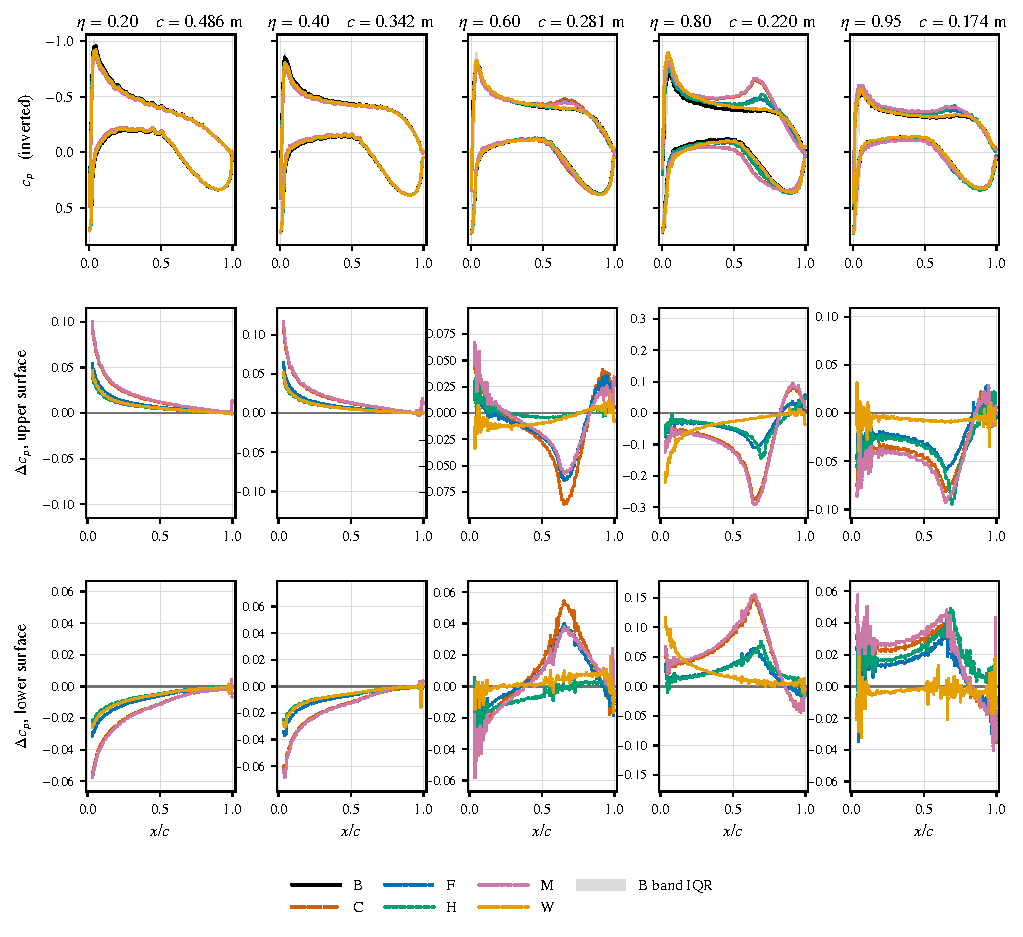
\includegraphics[width=\linewidth]{fig/fig_cp_sections_CR.pdf}
\caption{Surface pressure at five spanwise stations, $\eta = 0.20$ to $0.95$, Condition~CR, every
geometry at its own trim to $C_L = 0.428277635108$. The top row is $c_p$ on each case's own
freestream $q$, inverted, with the grey band the baseline's interquartile spread within the pooled
span band; the two lower rows are each candidate minus the baseline on the upper and lower
surfaces, drawn from $x/c = 0.03$ because forward of that the branch split and the span band are
ill-conditioned. $x/c$ is on the band's local chord, printed above each column.}
\label{fig:perf:cp}
\end{figure}

\begin{figure}[htbp]
\centering
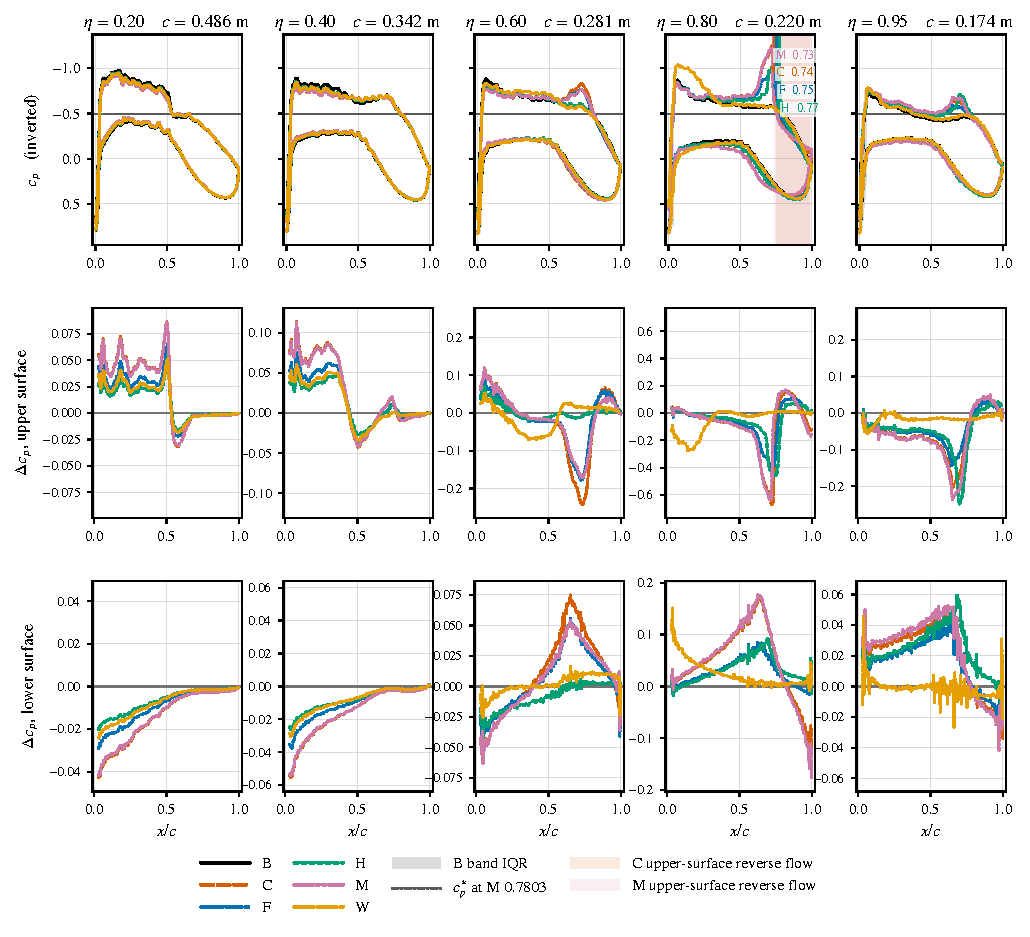
\includegraphics[width=\linewidth]{fig/fig_cp_sections_earlycruise.pdf}
\caption{Surface pressure at the same five stations, early cruise, every geometry at its own trim
to $C_L = 0.529297087450$; layout as Figure~\ref{fig:perf:cp}. The dashed line is the sonic
$c_p^{*}$, the tick marks at $\eta = 0.80$ locate each candidate's shock by its $x/c$, and the
shaded runs are where the upper-surface flow on C and M is reversed.}
\label{fig:perf:cp:ec}
\end{figure}

\begin{figure}[htbp]
\centering
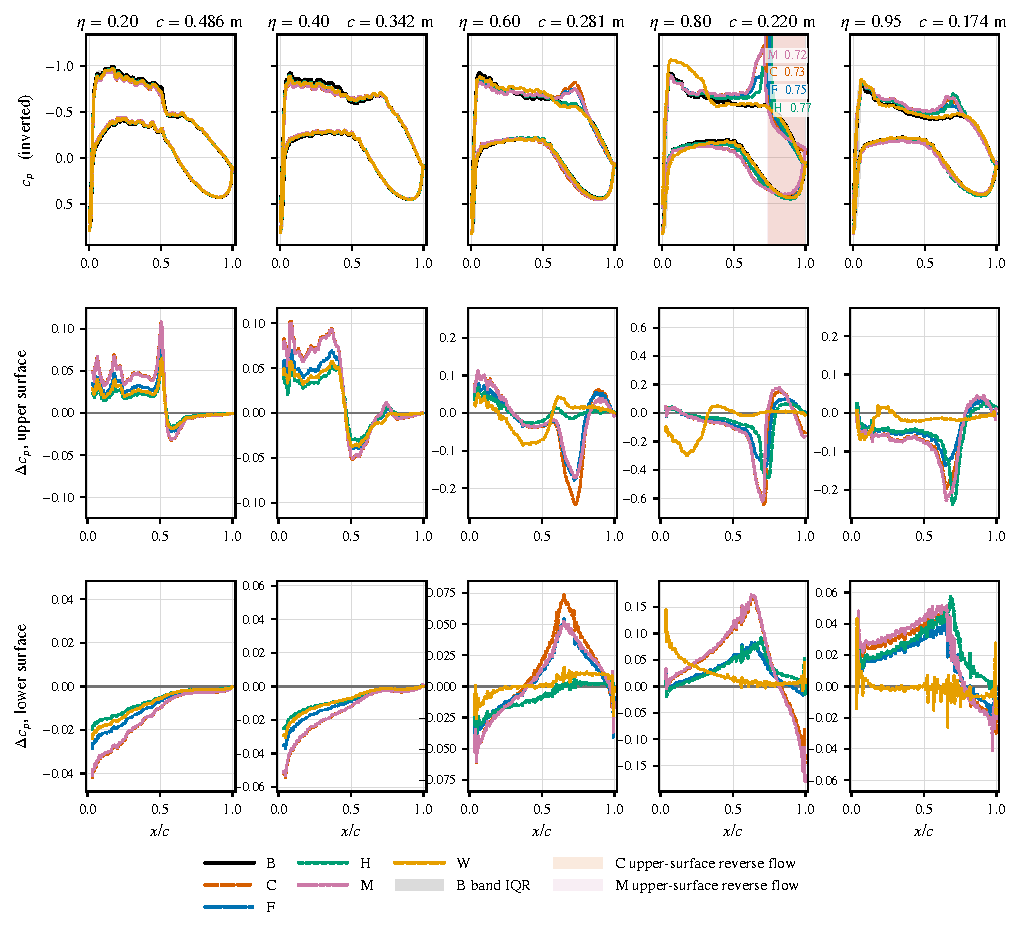
\includegraphics[width=\linewidth]{fig/fig_cp_sections_latecruise.pdf}
\caption{Surface pressure at the same five stations, late cruise, every geometry at its own trim
to $C_L = 0.544114800210$; layout as Figure~\ref{fig:perf:cp:ec}.}
\label{fig:perf:cp:lc}
\end{figure}
\textbf{Reading the skin-friction figures.} Condition~CR is wall resolved at $y^+ \approx 1$ with
kOmegaSST and cruise is wall modelled with Spalart-Allmaras, so $c_f$ is not equally resolved
between the two conditions and the two columns of each figure are read separately rather than
against one another. Neither $c_p$ nor $c_f$ carries a reference area.

\textbf{The plotted quantity and its sign.} The figures show
$c_{f,s} = m\,(\tau_w\!\cdot\!\hat{d})/q$, the \emph{freestream-aligned} component of wall shear,
with $\hat{d}$ taken from each case's own \texttt{forceCoeffs} drag direction. On this swept wing
that is not the section-normal component. OpenFOAM returns a negative wall shear for flow attached
in $+x$, so a calibrated sign multiplier $m$ is read from every file's own header, $m = -1$ on all
of them, and positive then plots as attached. It is therefore the \textbf{sign change} that
locates separation, never the magnitude. Lines are medians over $0.005c$ bins of the sampled band,
with at least five faces per bin. A band counts as a \emph{separated run} only when at least four
consecutive bins are negative, which is more than $2$~per~cent of local chord, so an isolated
negative bin is not read as separation. At $\eta = 0.95$ and $x/c > 0.875$ the curve is drawn in
grey because the aft bin there is band-averaged rather than resolved.

\textbf{What the ninety bands contain.} Over the $90$ (case, station) bands of the three
conditions, the largest reversed fraction on any upper surface is $25.3$~per~cent
(\texttt{LCM\_trim}, $\eta = 0.80$), and $31$ bands carry any reversed upper-surface face at all.
On the lower surface the largest is $0.474$~per~cent (\texttt{SWC\_trim}, $\eta = 0.20$); $56$
bands carry a trace, and those sit at the root junction and in the blunt trailing-edge base region
rather than being boundary-layer separation. The four bands that genuinely separate, C and M at
$\eta = 0.80$ at each cruise point, are named in Section~\ref{sec:perf:mechanism}.
\begin{figure}[htbp]
\centering
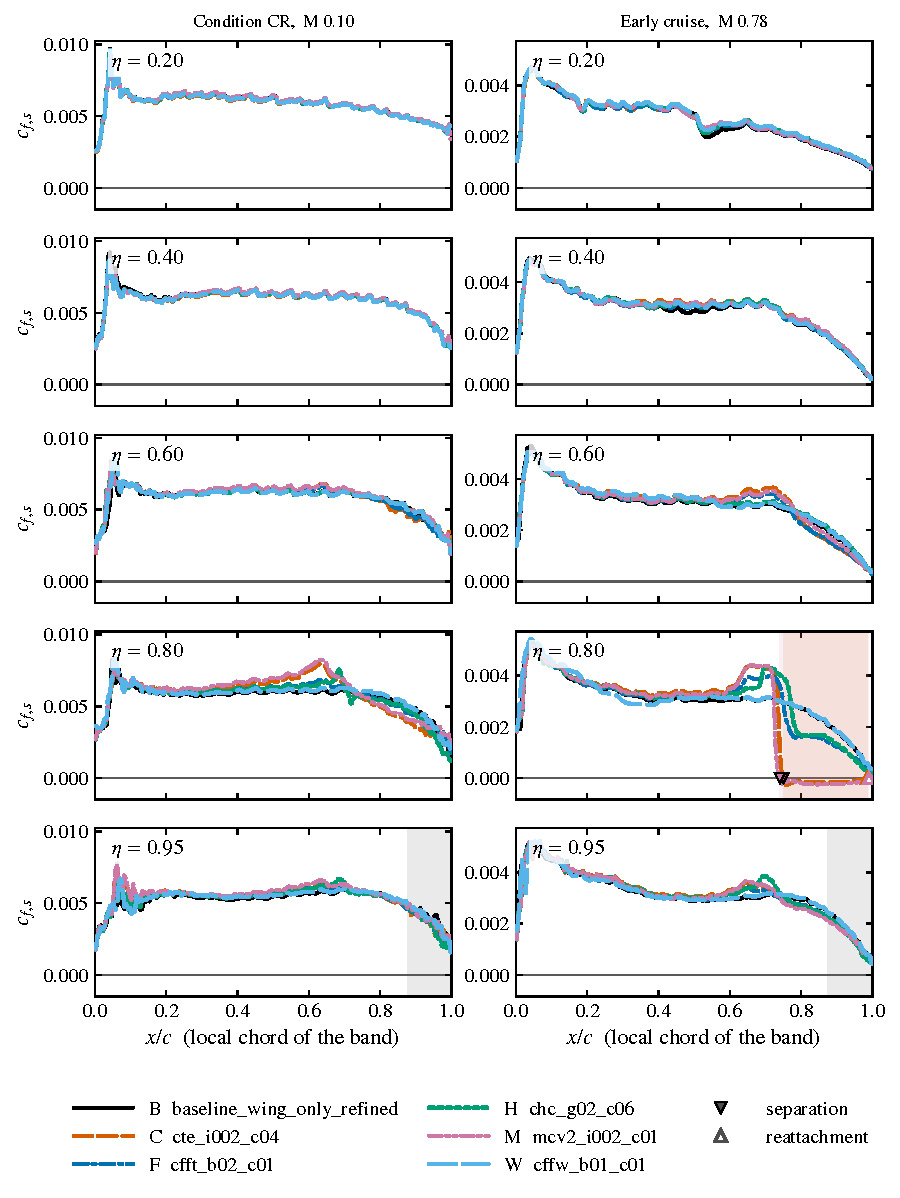
\includegraphics[width=\linewidth]{fig/fig_cf_sections_upper.pdf}
\caption{Signed skin friction $c_{f,s}$ at the same five stations, \textbf{upper} surface,
Condition~CR wall resolved on the left and early cruise wall modelled on the right, each geometry
at its own trim. Positive is attached and negative reversed, so it is the sign change and not the
magnitude that locates separation: the two separated runs at early cruise, C and M at
$\eta = 0.80$, are marked with their separation and reattachment stations. Late cruise separates
at the same two bands (Section~\ref{sec:app:sections:lc}). The
grey region at $\eta = 0.95$ is where the aft bin is band-averaged rather than resolved.}
\label{fig:perf:cf}
\end{figure}

\begin{figure}[htbp]
\centering
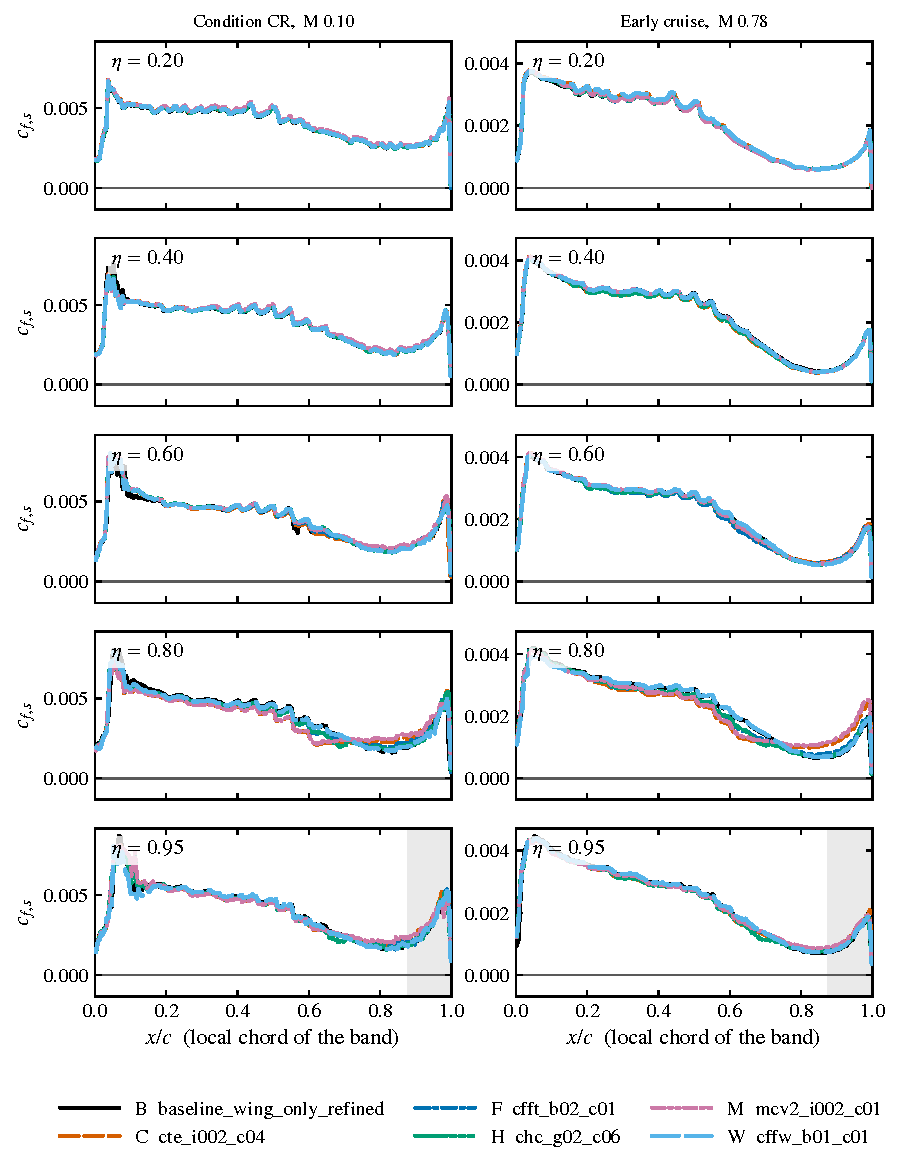
\includegraphics[width=\linewidth]{fig/fig_cf_sections_lower.pdf}
\caption{The same, \textbf{lower} surface. No lower-surface band carries a separated run at
either condition; the traces at the blunt trailing edge are the base region, not boundary-layer
separation.}
\label{fig:perf:cf:lower}
\end{figure}
\subsection{Condition CR, \texorpdfstring{$M = 0.10$, $C_L = 0.428277635108$}{M 0.10, CL 0.428277635108}}
\label{sec:app:sections:cr}

Nothing separates. Across all six geometries and all five stations the reversed fraction never
exceeds $0.25$~per~cent of faces in a band, and those faces sit at the blunt trailing edge and
the root junction, where they are present on the rigid baseline too. The six geometries lie
almost on top of one another: at $\eta = 0.60$ the upper-surface suction plateaus agree within
about $0.02$ in $-C_p$, and the morphing appears only aft of the hinge.

\subsection{Early cruise, \texorpdfstring{$M = 0.78$, $C_L = 0.529297087450$}{M 0.78, CL 0.529297087450}}
\label{sec:app:sections:ec}

At $M = 0.78$ the aft-camber candidates carry a recompression shock on the upper surface between
$x/c \approx 0.65$ and $0.78$ that is absent from the baseline. Two of them separate behind it,
and they are the two with the largest commanded camber.

At $\eta = 0.80$, C peaks at $-C_p = 1.279$ at $x/c = 0.716$ and M at $1.249$ at $x/c = 0.703$.
Both lose the boundary layer behind the shock and do not recover it before the trailing edge:
$23.3$~per~cent of C's upper-surface faces in that band are reversed, over $x/c = 0.743$ to
$0.992$, and $23.9$~per~cent of M's, over $x/c = 0.730$ to $0.997$, while both lower surfaces
reverse nowhere at all. M's shock is the stronger of the two, $\mathrm{d}c_p/\mathrm{d}(x/c) =
50.7$ against C's $45.7$, which follows its larger command: $A/c = 0.0350$ against C's $0.0337$. F
and H carry a weaker shock at a lower peak, $0.988$ at $x/c = 0.721$ and $1.027$ at
$x/c = 0.734$, and stay attached with zero reversed faces; F's command is $A/c = 0.0139$, two and
a half times smaller. W peaks forward, $1.074$ at $x/c = 0.067$, and has no aft shock at all. The
baseline peaks at $0.906$ at $x/c = 0.054$ and likewise has none.

This is the one place in the campaign where a candidate's flow is qualitatively different from
the baseline's rather than quantitatively so, and it is what makes C and M the two most expensive
candidates at cruise. It is local in span: at $\eta = 0.60$ and $0.40$ neither C nor M reverses a
single face, and at $\eta = 0.95$ each reverses one face, $0.010$~per~cent.

\subsection{Late cruise, \texorpdfstring{$M = 0.78$, $C_L = 0.544114800210$}{M 0.78, CL 0.544114800210}}
\label{sec:app:sections:lc}

Late cruise repeats early cruise station by station. At $\eta = 0.80$ C and M carry the strong
shock, $43.6$ at $x/c = 0.7325$ and $38.0$ at $0.7175$, peak at $-C_p = 1.248$ and $1.228$, and
separate behind it: $24.1$~per~cent of C's upper-surface faces reversed, over $x/c = 0.734$ to
$0.994$, and $25.3$~per~cent of M's, over $0.725$ to $0.997$, with both lower surfaces clean. F
and H carry the weaker shock, $16.1$ and $16.8$, and stay attached. W and the baseline have no aft
shock. Off $\eta = 0.80$ the picture is the early-cruise one: no reversal on C or M at
$\eta = 0.40$ and $0.60$, and one face each at $\eta = 0.95$.

\textbf{Provenance.} Sections are cut from each case's own \texttt{wingSurface.vtk} at its
converged iteration by \texttt{scripts/section\_slices\_from\_surface.py}, which also writes the
upper/lower flag from the per-face Newell normal, its sign calibrated per case against the more
negative mean $C_p$ at mid-chord and cross-checked against median $z$, refusing rather than
guessing if the two criteria disagree. The wind axes are the trimmed leg's own, read from its
\texttt{forceCoeffs} history in numeric order of the legs. The cruise surfaces were pulled from the
cluster with every file's checksum verified, and each section manifest records the source case,
the surface checksum and the extractor version. The figures are drawn by \texttt{fig/make\_cp.py}
and \texttt{fig/make\_cf.py}. The station files, their per-file headers ($q$, $p_\infty$, local
chord, \texttt{dragDir}, shear sign) and the extraction manifests are in
\texttt{data/sections\_welded/} for both cruise points, \texttt{data/sections\_r2/} for B, C, F,
H and W at Condition~CR and \texttt{data/sections\_nflag/} for M at Condition~CR, resolved per
case by \texttt{fig/section\_source.py}; the superseded set carrying the geometric split is
retained beside them in \texttt{data/sections/}.
